\chapter{Wave Fields}\label{ch:waves}

\section{Introduction}

In the previous Chapters~\ref{ch:potential} and \ref{ch:diffusion} we examined potential fields and diffusive fields, which describe how conserved quantities respond to spatial gradients under distinct assumptions about time. Potential fields arise when sources and fluxes are in instantaneous balance, while diffusive fields emerge when storage allows systems to evolve gradually toward equilibrium. Both classes redistribute structure smoothly and do not exhibit finite propagation speeds.

In this chapter we introduce a third and fundamentally different mode of behavior: wave propagation. Wave fields arise when conserved quantities are coupled to both restoring forces and inertia. Under these conditions, disturbances propagate at finite speeds, transport energy through the medium, and preserve structured information in time.

The wave equation governs a wide range of geophysical phenomena. These include seismic waves in solids, acoustic waves in fluids, electromagnetic waves (e.g., ground-penetrating radar), thermal waves driven by periodic forcing (e.g., climate and seasonal heat signals), and fluid waves associated with pressure and free-surface motion. Despite their differing physical origins, all wave phenomena share a common mathematical structure and a set of characteristic behaviors.

Unlike potential fields and diffusion, wave propagation does not inherently smooth spatial structure. Instead, waves transmit signals through the medium, often with attenuation and dispersion that depend on material properties. Finite travel times, reflections at boundaries, refraction due to spatial heterogeneity, diffraction around obstacles, and interference between waveforms are common features of all wave fields.

From a geophysical perspective, waves are uniquely powerful because they preserve spatial and temporal structure during propagation. Information is encoded in arrival times, amplitudes, phases, and waveforms rather than in static or time-averaged fields. As a result, wave-based observations form the foundation of seismology, radar methods, and many active-source and time-dependent imaging techniques.

The goal of this chapter is to develop physical intuition for wave behavior independent of any specific application. We examine how conservation laws, restoring forces, and inertia combine to produce the wave equation, explore the properties of wave solutions, and contrast wave propagation with the diffusive and steady-state behaviors encountered previously. These ideas provide the conceptual basis for seismic, electromagnetic, and fluid-wave methods developed later in the course.

\section{From conservation to wave motion}

Wave propagation emerges when conservation laws operate in the presence of both restoring forces and inertia. As in potential and diffusive fields, conservation of a physical quantity remains central. What distinguishes wave behavior is that the system resists motion through inertia and is driven back toward equilibrium by restoring forces rather than by diffusive smoothing.

To see this, consider a medium that can be displaced from equilibrium. A local disturbance produces a restoring force that acts to reverse the displacement. At the same time, inertia prevents the system from responding instantaneously. The resulting competition between restoring forces and inertia allows disturbances to propagate through the medium as waves.

From a conservation perspective, wave motion is most naturally associated with the conservation of momentum or energy rather than the direct conservation of a scalar quantity such as mass or heat. A local force imbalance leads to acceleration, not immediate transport or storage. This distinction is fundamental: in diffusion, imbalances drive fluxes that redistribute stored quantities, whereas in waves, imbalances drive motion that transports energy through the medium.

Restoring forces take different physical forms in different systems. In elastic solids, they arise from stress-strain relationships; in fluids, from pressure gradients; in electromagnetic waves, from the coupling between electric and magnetic fields. In all cases, the restoring force acts to oppose displacement from equilibrium.

Inertia provides the second essential ingredient. Without inertia, restoring forces would lead only to instantaneous relaxation, as in diffusion. Inertial resistance causes the system to overshoot equilibrium, producing oscillatory behavior. These oscillations allow energy to be transmitted through the medium rather than locally dissipated.

The presence of inertia introduces finite propagation speeds and causality. A disturbance at one location influences another only after sufficient time has elapsed for the wave to travel between them. This behavior stands in sharp contrast to both potential fields, which respond instantaneously, and diffusive fields, which respond everywhere immediately but only weakly at large distances.

Viewed in this light, wave propagation represents a third fundamental response to imbalance in physical systems:
\begin{itemize}
    \item potential fields enforce instantaneous balance,
    \item diffusion relaxes imbalance through gradual redistribution and storage,
    \item waves transport imbalance through oscillatory motion and energy flow.
\end{itemize}

In the next section, we make these ideas concrete by deriving the wave equation and examining how restoring forces and inertia combine to determine propagation speed and wave behavior.

\section{The wave equation}

The discussion in the previous section identified restoring forces and inertia as the essential ingredients required for wave propagation. When these ingredients are combined with conservation principles, the result is a governing equation that describes the propagation of disturbances through a medium at finite speed.

To illustrate this structure, we first consider a simplified case in which wave motion can be described by a single scalar field $\phi(\vb{x},t)$. This scalar form of the wave equation captures the essential physics common to many wave phenomena, including acoustic waves, electromagnetic waves in homogeneous media, and simplified elastic motion. More complex wave systems encountered in geophysics—particularly seismic waves in solids—require a vector or tensor description and are addressed separately.

The physical origin of the wave equation is presented in Box~\ref{box:wave_derivation}.  Here we summarize the key result.

When inertia resists acceleration and restoring forces act to oppose displacement, the evolution of the field $\phi$ is governed by
\[
    \pdv[2]{\phi}{t} = c^2 \laplacian \phi,
\]
where $c$ is the wave speed. This equation describes the propagation of disturbances without intrinsic smoothing or storage-driven relaxation. Instead, energy is transported through the medium by oscillatory motion.

The appearance of a second-order time derivative distinguishes wave propagation from diffusion. In diffusive systems, storage leads to gradual relaxation toward equilibrium, whereas in wave systems inertia allows disturbances to overshoot equilibrium and propagate. The resulting motion preserves structure over time and enforces causality through finite propagation speed.

\subsection{Scope and limitations}

The scalar wave equation provides a useful conceptual framework, but it does not capture the full richness of wave phenomena in elastic solids. In particular, seismic waves involve vector displacement fields and tensor relations between stress and strain. These lead to multiple wave modes, including compressional (P) waves, shear (S) waves, and surface waves, each with distinct propagation characteristics.

Rather than introduce this complexity here, we use the scalar wave equation to develop intuition for wave behavior common to all wave fields. The full elastic wave equation and the resulting diversity of seismic wave types are developed in detail in the seismology chapter.

\ntextbox{Physical origin of the wave equation}{
    Wave propagation arises from the interaction between inertia and restoring forces.  This can be illustrated using a simple one--dimensional medium in which a scalar field $\phi(x,t)$ describes displacement from equilibrium.

    \medskip
    \noindent\textbf{Inertia} \\
    A small element of the medium resists changes in motion according to Newton's second law. The inertial response is proportional to the second time derivative of the displacement,
    \[
        \text{force per unit volume} \;\propto\; \pdv[2]{\phi}{t}.
    \]

    \medskip
    \noindent\textbf{Restoring force}\\
    Displacement from equilibrium produces a restoring force that tends to return the system to its original state. For small deformations, this restoring force is proportional to spatial curvature in the displacement,
    \[
        \text{restoring force per unit volume} \;\propto\; \laplacian \phi.
    \]

    \medskip
    \noindent\textbf{Balance of forces}\\
    Equating inertial and restoring terms leads to
    \[
        \pdv[2]{\phi}{t} = c^2 \laplacian \phi,
    \]
    where the wave speed $c$ depends on the ratio of the restoring stiffness of the medium to its inertial mass density.

    \medskip
    \noindent This equation describes the propagation of disturbances at finite speed without diffusive smoothing. Energy is conserved locally and transported through the medium by oscillatory motion.
}{core}\label{box:wave_derivation}

\section{Finite propagation speed and wave velocity}

A fundamental distinction between wave fields and both potential and diffusive fields is the existence of a finite propagation speed. Disturbances do not influence the entire domain instantaneously; instead, information and energy travel through the medium at a characteristic velocity determined by material properties.

Wave velocity arises from the balance between restoring forces and inertia. Strong restoring forces increase wave speed, while larger inertia slows propagation. This relationship is general: regardless of the physical nature of the wave, velocity reflects the ratio of stiffness to mass or storage.

The parameter $c$ has units of velocity and represents the speed at which disturbances propagate (Table~\ref{tab:velocity}). Unlike diffusivity, wave speed does not introduce smoothing. Ideal wave solutions preserve waveform shape during propagation.
\begin{table}[bth]
    \centering
    \caption{Wave velocity in common geophysical and geoscientific systems}
    \label{tab:wave_velocity}
    \begin{tabularx}{\textwidth}{lXYX}
        \toprule
        \textbf{System} &
        \textbf{Wave type} &
        \textbf{Velocity expression} &
        \textbf{Controlling properties} \\
        \midrule
        Elastic solids
        & Seismic body waves
        & $c \sim \sqrt{\mathrm{elastic modulus}/\rho}$
        & Bulk/shear modulus, density \\

        Elastic solids
        & Seismic surface waves
        & $c \lesssim c_S$
        & Near-surface structure, layering \\

        Fluids
        & Acoustic waves
        & $c = \sqrt{K/\rho}$
        & Bulk modulus, density \\

        Electromagnetics
        & EM waves (GPR, radar)
        & $c = 1/\sqrt{\mu\varepsilon}$
        & Permeability, permittivity \\

        Thermal systems
        & Thermal waves
        & $c_{\mathrm{phase}} = \omega/k$
        & Diffusivity, forcing frequency \\

        Fluid surfaces
        & Gravity waves
        & $c \sim \sqrt{g\lambda}$
        & Gravity, wavelength \\

        Porous media
        & Pressure waves
        & $c \sim \sqrt{K_{\mathrm{eff}}/\rho_{\mathrm{eff}}}$
        & Frame rigidity, fluid coupling \\
        \bottomrule
    \end{tabularx}
\end{table}

Finite propagation speed introduces causality. A point in space responds to a disturbance only after sufficient time has elapsed for the wave to travel from the source. Travel times, arrival sequences, and waveform evolution therefore carry direct information about the medium through which the wave has passed.


\section{General properties of wave propagation}

Solutions of the wave equation exhibit a set of characteristic behaviors that are common to all wave phenomena, regardless of their physical origin.  The wave equation admits a rich set of solutions that describe how disturbances interact with material boundaries, propagate through heterogeneous media, and transport energy. These properties arise directly from the combination of restoring forces and inertia and distinguish wave fields from both steady-state potential fields and diffusive systems.  Although the physical interpretation of waves varies across geophysics, the same mathematical relationships govern their behavior. In this section we introduce a set of general concepts and equations that apply broadly to seismic, acoustic, electromagnetic, thermal, and fluid waves.

\subsection{Impedance and wave interaction with boundaries}

A central quantity in wave propagation is the \emph{wave impedance}, which measures how a medium resists motion or field oscillation. Impedance combines inertial and restoring properties and depends on the physical system. For a wide class of scalar waves, it may be written schematically as
\[
    Z = \frac{\text{restoring strength}}{\text{particle or field velocity}}.
\]

At a boundary separating two media, impedance controls how wave energy is partitioned between reflection and transmission. For normally incident waves, the amplitude reflection and transmission coefficients can be written in the general form
\[
    R = \frac{Z_2 - Z_1}{Z_2 + Z_1}, \qquad
    T = \frac{2 Z_2}{Z_1 + Z_2},
\]
where $Z_1$ and $Z_2$ are the impedances of the incident and transmitted media, respectively. These expressions apply to acoustic waves, electromagnetic waves, and elastic waves under appropriate definitions of impedance.

Large impedance contrasts lead to strong reflections, while small contrasts favor transmission. This simple result underlies reflection seismology, radar sensing, and many scattering phenomena.

In systems where multiple wave modes are possible—most notably in elastic solids—incident wave energy can be partitioned among reflected and transmitted modes with different polarizations and speeds. While the scalar wave equation does not capture this behavior, the underlying principles of impedance contrast and slowness conservation remain valid. The detailed treatment of mode conversion is reserved for the seismology chapter.

\subsection{Reflection and refraction: Snell's law}

When waves encounter a planar interface at an angle, their directions of propagation change in a way constrained by phase continuity along the boundary.  This requirement leads to Snell's law, which relates angles of incidence, reflection, and transmission (Figure~\ref{fig:wave_phenomena}).
\begin{figure}[bth]
    \centering
    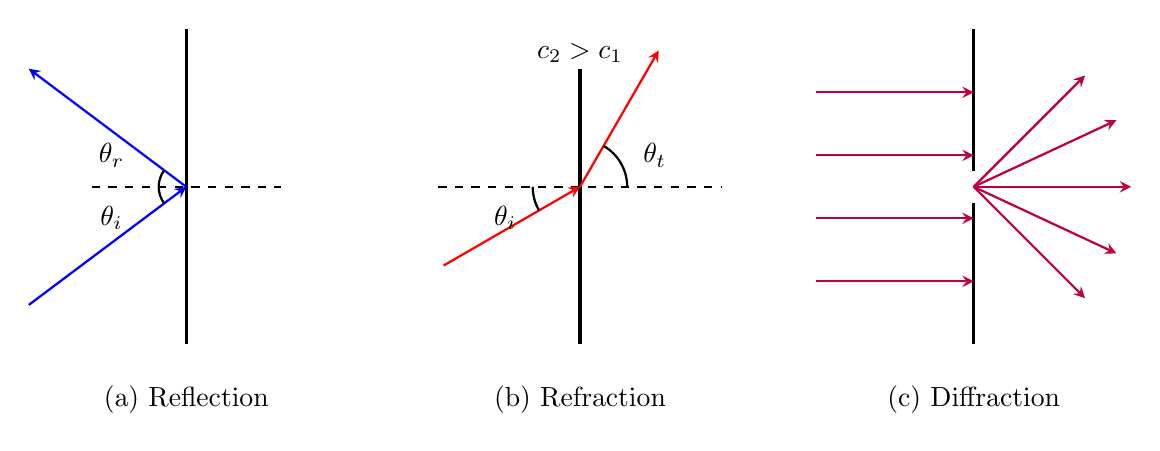
\begin{tikzpicture}[scale=1.0, thick, >=stealth]

    %========================
    % Panel (a): Reflection
    %========================
    \begin{scope}[shift={(0,0)}]
        % Boundary
        \draw[very thick] (0,0) -- (0,4);
        %\node[rotate=90] at (-0.45,2) {Boundary};

        % Normal
        \draw[dashed] (-1.2,2.0) -- (1.2,2.0);
        %\node at (1.35,2.5) {Normal};

        % Incident wave
        \draw[->, blue] (-2,0.5) -- (0,2.0);
        %\node[blue] at (-1.6,1.2) {Incident};

        % Reflected wave
        \draw[->, blue] (0,2.0) -- (-2,3.5);
        %\node[blue] at (-1.6,3.7) {Reflected};

        % Angles
        \draw (-0.35,2.0) arc[start angle=180,end angle=217,radius=0.35];
        \node at (-0.95,1.6) {$\theta_i$};

        \draw (-0.35,2.0) arc[start angle=180,end angle=143,radius=0.35];
        \node at (-0.95,2.4) {$\theta_r$};

        % Label
        \node at (0,-0.7) {(a) Reflection};
    \end{scope}

    %========================
    % Panel (b): Refraction (explicit angles)
    %========================
    \begin{scope}[shift={(5,0)}]

        % Interface (vertical)
        \draw[very thick] (0,0) -- (0,3.5);

        % Normal (horizontal, pointing to the right)
        \draw[dashed] (-1.8,2) -- (1.8,2);
        %\node at (2.0,2) {Normal};

        % Incident ray: -30° from normal
        % Direction = 180 - 30 = 150 degrees
        \draw[<-, red] (0,2) -- ++(210:2);
        %\node[red] at (-1.7,2.7) {Incident};

        % Transmitted ray: +60° from normal
        % Direction = 0 + 60 = 60 degrees
        \draw[->, red] (0,2) -- ++(60:2);
        %\node[red] at (1.6,3.2) {Refracted};

        % Incident angle theta_i (between normal and incident ray)
        \draw (-0.6,2)
            arc[start angle=180,end angle=210,radius=0.6];
        \node at (-0.95,1.6) {$\theta_i$};

        % Transmitted angle theta_t (between normal and refracted ray)
        \draw (0.6,2)
            arc[start angle=0,end angle=60,radius=0.6];
        \node at (0.95,2.4) {$\theta_t$};

        % velocity labels
        \node at (0,3.7) {$c_2 > c_1$};

        % Panel label
        \node at (0,-0.7) {(b) Refraction};

    \end{scope}

    %========================
    % Panel (c): Diffraction
    %========================
    \begin{scope}[shift={(10,0)}]
        % Barrier with aperture
        \draw[very thick] (0,0) -- (0,1.8);
        \draw[very thick] (0,2.2) -- (0,4);
        %\node[rotate=90] at (-0.45,2) {Barrier};

        % Incident waves
        \foreach \y in {0.8,1.6,2.4,3.2} {
            \draw[->, purple] (-2,\y) -- (0,\y);
        }
        %\node[purple] at (-1.6,0.5) {Incident};

        % Diffracted waves
        \foreach \angle in {-45,-25,0,25,45} {
            \draw[->, purple] (0,2) -- ++(\angle:2);
        }
        %\node[purple] at (1.7,3.5) {Diffracted};

        % Label
        \node at (0,-0.7) {(c) Diffraction};
    \end{scope}

    \end{tikzpicture}
    \caption{Schematic illustration of (a) reflection, (b) refraction, and (c) diffraction of waves.  Dashed lines indicate the surface normal relevant to Snell's law.  Geometry is schematic and not to scale.}
    \label{fig:wave_phenomena}
\end{figure}

For reflection, the angle of incidence equals the angle of reflection, both
measured from the surface normal,
\[
    \theta_i = \theta_r .
\]

For transmission (refraction), the angles are related by
\[
    \frac{\sin \theta_i}{c_1} = \frac{\sin \theta_t}{c_2},
\]
where $c_1$ and $c_2$ are the wave speeds in the two media. This form emphasizes that refraction arises from changes in propagation speed, not from changes in frequency.

A more general and widely transferable form of Snell's law expresses conservation of horizontal slowness,
\[
p = \frac{\sin \theta}{c},
\]
which remains constant across interfaces. This formulation applies equally to seismic, acoustic, and electromagnetic waves and provides a natural bridge to ray theory and travel-time analysis developed later.

\subsection{Diffraction and wavelength effects}

Waves also exhibit diffraction: the tendency to spread laterally when encountering obstacles or apertures comparable in size to the wavelength. Diffraction places a fundamental limit on spatial resolution and ensures that wave energy is not confined to perfectly sharp paths.

As a result, wave behavior depends not only on geometry and boundaries, but also on the relationship between wavelength and the scale of heterogeneity in the medium.  This scale dependence will reappear when discussing the resolving power of wave-based geophysical methods.

\subsection{Superposition and interference}

The wave equation is linear, which allows solutions to be superposed. When multiple waves occupy the same region of space, their displacements add. This superposition can produce constructive and destructive interference, giving rise to complex spatial and temporal patterns even in simple media.

Interference underlies many familiar wave phenomena, including beat patterns, standing waves, and resonances. In geophysics, interference plays an important role in shaping observed waveforms and spectra.


\section{Energy transport, attenuation, and dispersion}

Waves transport energy through a medium rather than redistributing it locally, but real geophysical materials do not transmit energy without loss or modification. As waves propagate, their amplitudes and frequency content evolve due to a combination of geometric effects, intrinsic dissipation, and scattering.

\subsection{Attenuation and Spherical Spreading}
In an ideal, lossless medium, the wave equation conserves energy. Energy is carried by the oscillatory motion of the medium or field and propagates at the group velocity. This transport allows waves to convey structured information over long distances without intrinsic smoothing, in contrast to diffusion.  The energy flux associated with a wave is proportional to the square of its amplitude, which makes amplitude a sensitive carrier of information about the propagation environment (Box~\ref{box:information}).

Ideal wave equations conserve energy, but real materials dissipate it. Attenuation describes the loss of wave amplitude due to intrinsic dissipation (e.g., viscosity, anelasticity, electrical resistance) and scattering. A common mathematical representation of attenuation is an exponential decay with distance,
\[
    A(x) = A_0\, e^{-\alpha x},
\]
where $\alpha$ is the attenuation coefficient. Attenuation reduces amplitudes but does not intrinsically alter propagation speed.

It is important to distinguish attenuation from diffusion. Diffusion irreversibly smooths structure, whereas attenuation reduces amplitude while preserving waveform shape over short distances.

Even in the absence of attenuation, wave amplitudes decrease as energy spreads over increasing area or volume. For point sources in three dimensions, spherical spreading leads to
\[
    A(r) \propto \frac{1}{r},
\]
while cylindrical spreading leads to $A(r) \propto r^{-1/2}$. Geometric spreading is a purely kinematic effect and applies to all wave types.

\subsection{Dispersion, Phase and Group Velocity}
A medium is dispersive if wave speed depends on frequency. In dispersive systems, different frequency components of a signal propagate at different velocities, causing waveforms to change shape with distance.  Dispersion is described through the relationship between angular frequency $\omega$ and wavenumber $k$. The phase and group velocities,
\[
    c_p = \frac{\omega}{k}, \qquad c_g = \frac{d\omega}{dk},
\]
may differ substantially in dispersive media.

The phase velocity $c_p$ describes the speed of constant phase (e.g., wave crests), while the group velocity $c_g$ describes the speed at which energy and information propagate.  The distinction between phase and group velocity is essential for interpreting wave packets, dispersion, and frequency-dependent travel times. These ideas will reappear in later chapters in the context of seismic surface waves, guided waves, and electromagnetic propagation.

Dispersion plays a critical role in surface waves, guided waves, electromagnetic propagation in layered media, and thermal or diffusive “wave-like” responses under periodic forcing.

\ntextbox{Memory and information in diffusive and wave systems}{
    When we describe diffusive and wave systems as having different degrees of memory or information content, we are not using metaphorical language. We are describing how much of a system's past or spatial structure remains encoded in observable signals as they propagate through a medium.

    \medskip
    \noindent\textbf{Memory in diffusive systems}\\
    Diffusive systems possess limited and rapidly degrading memory. Information about an initial disturbance is retained only transiently and only in a highly smoothed, integrated form. As diffusion proceeds, local gradients relax, and fine-scale structure is irreversibly erased.  In practical terms, this means that a diffusive signal carries information primarily about:
    \begin{itemize}
        \item the gross distribution of sources and boundaries,
        \item the integrated properties of the medium,
        \item and the time elapsed since perturbation.
    \end{itemize}

    Early-time diffusive responses may retain some sensitivity to local structure, but this sensitivity decays rapidly. At late times, different initial conditions that share similar large-scale properties become indistinguishable. Diffusion therefore acts as both a spatial and temporal low-pass filter, progressively losing information about the detailed path taken by energy, mass, or charge.  This behavior is why diffusive methods emphasize bulk properties and why inverse problems based on diffusion are strongly non-unique and increasingly ill-posed at late times.

    \medskip
    \noindent\textbf{Memory and information in wave systems}\\
    Wave systems behave fundamentally differently. Because waves propagate via oscillatory motion rather than gradual relaxation, they preserve structured information as they travel. This information is not stored locally but is carried by the wave itself.  In geophysics, information about the medium and the propagation path is encoded in multiple observable attributes of a wavefield, including:

    \begin{itemize}
        \item travel times, which reflect integrated velocity along the propagation path;
        \item relative arrival times of different phases, which constrain structure and layering;
        \item amplitude, which reflects geometrical spreading, attenuation, and impedance contrasts;
        \item phase and polarity, which encode boundary interactions and mode conversions;
        \item wavelet shape and frequency content, which reflect dispersion and attenuation; and
        \item coda length and complexity, which record scattering and multipathing. 
    \end{itemize}

    A key point is that this information is path-dependent. As a wave travels, it is continually modified by the material it encounters, and these modifications accumulate coherently rather than being smoothed away. In this sense, a wavefield retains a memory of its history: the source wavelet is convolved with the impulse response of the Earth along each propagation path.  This is why waves are so powerful for imaging. Even a single waveform can contain multiple, overlapping pieces of information about source location, medium structure, and boundary geometry.

    \medskip
    \noindent\textbf{Causality and information transport}\\
    The difference in memory between diffusive and wave systems is closely tied to causality.
    
    Diffusive systems respond everywhere immediately, but only weakly at large distances. Information spreads, but without a sharp arrival time or a clear causal sequence.
    
    Wave systems exhibit finite propagation speed. Information arrives at distinct times, in ordered sequences, allowing causal interpretation: one feature happened before another.  This temporal ordering is essential for extracting directional and geometric information, such as travel paths, reflectors, and interfaces.

    \medskip
    \noindent\textbf{Why this distinction matters in geophysics}\\
    Understanding memory and information content clarifies why different geophysical methods are suited to different questions.

    Diffusion-based observations are best for estimating bulk properties, long-term evolution, and integrated structures.  Wave-based observations are best for recovering geometry, layering, and localized heterogeneity.

    Neither is “better” in an absolute sense—they answer different questions because they retain different kinds of information.
}{aside}\label{box:information}


\section{Potential, diffusive, and wave fields: a unified perspective}
With the introduction of wave propagation, we can now place potential fields, diffusive fields, and wave fields within a single conceptual framework. All three arise from conservation laws combined with constitutive relations, but they differ in the physical mechanisms through which imbalance is resolved.

Potential fields (elliptic) phenomena enforce instantaneous balance between sources and fluxes. They exhibit global sensitivity, intrinsic smoothness, and strong non-uniqueness, with no characteristic time scale.

Diffusive fields (parabolic) resolve imbalance through gradual redistribution and storage. They introduce memory loss, smoothing, and a characteristic time-length scale $\ell \sim \sqrt{\kappa t}$. In the long-time limit, the diffusive field approaches elliptic behavior.

Wave fields (hyperbolic) resolve imbalance through oscillatory motion mediated by inertia and restoring forces. They exhibit finite propagation speed, preserve structured information, and transport energy through the medium.  The wave equation also differs in that it does not admit a steady-state or diffusive limit: energy propagates rather than relaxes.

These distinctions reflect differences in mathematical character rather than differences in conservation principles.

The three field types also differ fundamentally in how information is encoded and transmitted:
\begin{itemize}
    \item potential fields integrate information globally and do not encode causal ordering;
    \item diffusive fields partially retain information at early times but progressively forget it; while
    \item wave fields preserve path-dependent, time-ordered information in amplitudes, phases, and waveforms.
\end{itemize}
This hierarchy explains why different geophysical methods are sensitive to different aspects of subsurface structure and why combining methods can reduce ambiguity.

The essential differences can be summarized schematically:
\begin{align*}
    \laplacian{\phi} &= s && \text{(potential fields)} \\
    \pdv{\phi}{t} &= \kappa \laplacian{\phi} && \text{(diffusion)} \\
    \pdv[2]{\phi}{t} &= c^2 \laplacian{\phi} && \text{(waves)}
\end{align*}
The progression from elliptic to parabolic to hyperbolic equations reflects increasing dynamical complexity and increasing information retention.

\section{Connection to geophysics}
Wave propagation is central to many geophysical and geoscientific methods, precisely because waves preserve information about structure, geometry, and material properties along their propagation paths.
In the Earth, wave phenomena arise in many contexts:
\begin{itemize}
    \item seismic waves in elastic solids,
    \item acoustic waves in fluids and the atmosphere,
    \item electromagnetic waves used in radar and remote sensing,
    \item periodic temperature changes at Earth's surface or at the base of the oceans,
    \item surface and gravity waves in oceans and rivers,
    \item pressure waves in porous and fractured media.
\end{itemize}

Although these systems involve different physical variables, they share common governing principles and mathematical structure.

\subsection{Imaging and inference}
Wave-based methods excel at resolving geometry. Travel times constrain velocity and layer thickness, amplitudes reveal impedance contrasts and attenuation, and waveform shapes encode dispersion and scattering. Reflections, refractions, and diffractions provide complementary constraints on boundaries and heterogeneities.

Because waves retain memory of their propagation history, inverse problems based on wave data are typically better constrained than those based solely on potential or diffusive fields, though they remain computationally challenging.

\subsection{Relationship to later chapters}
The scalar wave equation and general properties introduced here provide the foundation for later chapters on seismology, radar methods, and electromagnetic wave propagation. In those chapters, the simplified framework developed here will be extended to include: vector and tensor fields, multiple wave modes, mode conversion and anisotropy, frequency-dependent attenuation and dispersion.

By establishing the common physics of wave propagation early, later method-specific developments can focus on interpretation rather than rederiving fundamental concepts.

Together with potential and diffusive fields, wave fields complete the triad of fundamental geophysical responses to imbalance. Understanding how and why these different field types behave as they do is essential for selecting appropriate methods, interpreting observations, and integrating multiple datasets into coherent models of the Earth.
